\documentclass[11pt,a4paper]{article}
\usepackage[T1]{fontenc}
\usepackage[utf8]{inputenc}
\usepackage{mathpazo}
\usepackage[scaled=0.92]{helvet}
\usepackage{microtype}
\usepackage[left=25mm,right=25mm,top=23mm,bottom=24mm]{geometry}
\usepackage{amsmath,amssymb,bm}
\usepackage{graphicx}
\usepackage{booktabs,array}
\usepackage{float}
\usepackage[font=small,labelfont=bf,labelsep=period,skip=5pt]{caption}
\usepackage{xcolor}
\usepackage[framemethod=default]{mdframed}
\usepackage[colorlinks=true,linkcolor=black,urlcolor=black,citecolor=black]{hyperref}
\usepackage{parskip}
\linespread{1.04}
\graphicspath{{../fig/}}
\definecolor{boxbg}{HTML}{F4F3EF}
\definecolor{rule}{HTML}{C3C2B7}
\captionsetup[figure]{name=Fig.}
\newcommand{\widefig}[1]{\noindent\makebox[\textwidth][c]{\includegraphics[width=7.16in]{#1}}}
\newcommand{\qL}{\hat q_{L,n}}
\newcommand{\qR}{\hat q_{R,n}}
\newcommand{\dq}{\Delta q}
\newcommand{\so}{\sigma_o}
\newcommand{\code}[1]{\texttt{#1}}
\setlength{\abovedisplayskip}{7pt}
\setlength{\belowdisplayskip}{7pt}

\begin{document}

{\sffamily\bfseries\LARGE Signal-to-noise ratio of the sound input\\[2pt] to the Sonoro ring attractor\par}
\vspace{4pt}
{\sffamily\large Experiment A1 of 16 November 2026: ten runs, A1\_02 left out\par}
\vspace{2pt}
{\small Prepared for Sindiso Mkhatshwa, 17 November 2026. Code, tables and figures are in \code{snr\_analysis/} of the repository.\par}
\vspace{6pt}

\begin{mdframed}[backgroundcolor=boxbg,linecolor=rule,linewidth=0.6pt,innertopmargin=8pt,innerbottommargin=8pt,innerleftmargin=10pt,innerrightmargin=10pt]
\textbf{The answer.} In the convention of the ICRA submission, where the sample of each target's quality carries
independent noise $\eta$ and the per-sample signal-to-noise ratio is $D=\dq/\eta$, the sound input at the start
of a run has
\[
D \approx 3.4\text{ to }3.8 \;\;\text{(right speaker at 0.7)}, \qquad D \approx 6.3\text{ to }6.4 \;\;\text{(right speaker at 0.6)},
\]
with the left speaker at 1. Each pair comes from two independent ways of separating signal from noise, and they
agree. The signal, the mean difference between the two lobes of the ring input, is 13\,\% and 19\,\% of the taller
lobe. The noise is 4 to 5\,\% of the taller lobe per control cycle. These ratios are 3 to 26 times those of the ICRA
grid ($D=0.25$, $0.5$, $1$).

The ratio does not stay put during a run, because the signal depends on where the robot is. With the right
speaker at 0.7 the signal changes sign seven to eleven cycles before the robot turns: the right lobe is then the
taller one by 12 to 13\,\%, and $D\approx-5$ to $-9$. That is why four of those five runs went to the quieter speaker. In all ten runs the robot turned to the lobe that was taller in the last samples before the turn. A bias of the
input that depends on the robot's position set the outcomes; the noise was too small to change them.
\end{mdframed}

\section{What the ring receives}

The two speakers chirp in turn, the left one on even seconds and the right one on odd seconds (5\,ms,
0.5 to 3.5\,kHz). In each control cycle the robot stands still and listens for 3\,s. During that time it repeatedly
takes the loudest 20\,ms of the latest 0.3\,s of sound and computes a DMAS-CF response $S_{n,m}(\theta_i)$ in
120 directions $\theta_i$. Of the measurements $m$ above 35\,dB the controller keeps, for each direction, the
largest response; it then rescales the result between its minimum and maximum and multiplies by 0.19. The
vector fed to the ring in cycle $n$ is therefore
\begin{equation}
\bm{h}_n = 0.19\,\frac{\bm{a}_n-\min_i a_{n,i}}{\max_i a_{n,i}-\min_i a_{n,i}},\qquad
a_{n,i}=\max_m S_{n,m}(\theta_i). \label{eq:h}
\end{equation}
A 20-ms measurement holds one chirp, so $\bm{h}_n$ has one lobe for each speaker (Fig.~\ref{fig:input}a). I write
$\qL$ and $\qR$ for the heights of the left and right lobes in units of the taller one, that is, of $h/0.19$.
The lobes stand clear of each other: at the closest separation, $48^\circ$, one lobe has fallen to 0.3 of its peak
where the other peaks. The heights are read at the two maxima and refined with a parabola through three bins.

The rescaling in \eqref{eq:h} sets the taller lobe to exactly 1. A cycle therefore delivers one number about the
two speakers, the ratio
\[
\rho_n=\qR/\qL .
\]
How loud the chirps were, and how much each lobe fluctuated on its own, is not in the log.

The log does contain exactly what the ring was given. The controller seeds its random generator with 300, so
the spins of every cycle can be recomputed from the logged $\bm{h}_n$ alone. Doing so reproduces all 105\,000
logged spins of the ten runs without a single difference. The ring code and parameters in the repository are
therefore those that ran, and since the ring started every run from the same seed, the runs differ only through
their input.

\begin{figure}[t]
\widefig{fig1_input_and_arena.pdf}
\caption{\textbf{(a)} The input $\bm{h}_n/0.19$ in three cycles of run A1\_08. L and R mark the lobes of the left
and right speakers; their heights are the samples $\qL$ and $\qR$. The taller lobe is always 1. \textbf{(b)} Paths of
the nine tracked runs (A1\_01 was not tracked). The robot starts 1.24\,m from the left and 1.21\,m from the right
speaker and turns after 47 to 55 cycles, 0.68\,m from both.}
\label{fig:input}
\end{figure}

\section{The definition, in the terms of the ICRA paper}

In the sensory model of the ICRA submission each target $k$ gives, at every sample, a noisy quality
$\hat q_k=q_k+\eta\,\xi_k$ with independent standard normal $\xi_k$. The evidence in a sample is the difference
$o=\hat q_1-\hat q_2$, which is normal with mean $\dq=q_1-q_2$ and standard deviation $\so=\sqrt2\,\eta$. The
per-sample signal-to-noise ratio and the probability that a sample has the right sign are
\begin{equation}
D=\frac{\dq}{\eta}=\frac{\sqrt2\,\dq}{\so},\qquad p=\Phi\!\left(\frac{D}{\sqrt2}\right). \label{eq:D}
\end{equation}

For the robot the sample of cycle $n$ is
\begin{equation}
o_n=\qL-\qR=\begin{cases}1-\rho_n, & \rho_n\le 1,\\[2pt] 1/\rho_n-1, & \rho_n>1,\end{cases} \label{eq:o}
\end{equation}
positive when the lobe of the left speaker, the louder one by design, is the taller. The robot moves, and what it
hears depends on where it is, so I write
\begin{equation}
o_n=\dq(\bm{x}_n)+\varepsilon_n ,\qquad D(\bm{x})=\frac{\sqrt2\,\dq(\bm{x})}{\so(\bm{x})}, \label{eq:model}
\end{equation}
where $\bm{x}_n$ is the pose of the robot in cycle $n$. The signal $\dq(\bm{x})$ is the mean sample at that pose,
and the noise $\so$ is the standard deviation of $\varepsilon_n$, the scatter of the samples about that mean.

Because the taller lobe is fixed at 1, all the scatter of $o_n$ sits in the shorter lobe, which the paper's model
does not assume. The noise of each target separately cannot be recovered; only $\so$ can. The value
$\eta=\so/\sqrt2$ used in \eqref{eq:D} is the equal noise on both targets that would give the same scatter of the
difference, which is what a decision between the two depends on. I took the convention $D=\dq/\eta$ from the
pre-registration of 23 October; under any other convention the quantity to carry over is
$d'=\dq/\so=D/\sqrt2$, which is also in \code{snr\_table.csv}.

\section{Two routes from the samples to signal and noise}

Because $\dq$ changes along a run, it is not the plain mean of the samples, and $\so$ is not their plain standard
deviation. The mean has to be separated from the scatter. I do it in two ways that rest on different
assumptions and use different data.

\textbf{Route A: regression on the measured geometry.} The height of a lobe is the product of the strength of
its source, a function of the distance to it, and the gain of the microphone array in its direction. The logarithm of
the ratio of the two lobes is then a sum of terms, and for $\ell_n=\ln\rho_n$ I fit
\begin{equation}
\ell_n=c_a+s(\alpha_n)+\gamma(\alpha_n)\,\ln\frac{d_{L,n}}{d_{R,n}}+e_n . \label{eq:routeA}
\end{equation}
Here $a$ is the level of the right speaker (0.7 or 0.6), $\alpha_n$ is the angle between the two lobes, read from
$\bm{h}_n$, and $d_{L,n}$, $d_{R,n}$ are the distances from the robot to the two speakers, from Qualisys. The
separation $\alpha$ grows steadily from $48^\circ$ to about $100^\circ$ as the robot advances, and I use it as the
coordinate along the approach: $s(\alpha)=a_1z+a_2z^2+a_3z^3$ and $\gamma(\alpha)=\gamma_0+\gamma_1z$ with
$z=(\alpha-70^\circ)/25^\circ$. The seven parameters are fitted with Huber weights to the 449 tracked samples
taken before the turn. With $\hat\ell_n$ the fitted value and $o(\ell)$ the map \eqref{eq:o}, the signal, noise and
ratio in a window $W$ of cycles are
\begin{equation}
\dq_A=\big\langle o(\hat\ell_n)\big\rangle_W,\qquad
\sigma_A^2=\big\langle\,[\,o_n-o(\hat\ell_n)\,]^2\big\rangle_W,\qquad
D_A=\frac{\sqrt2\,\dq_A}{\sigma_A}. \label{eq:A}
\end{equation}

\textbf{Route B: successive differences.} This route needs \code{ringStats} only. The robot advances 13\,mm
per cycle, a tenth of the shortest wavelength in the 1 to 2.8\,kHz band the controller listens to, so the mean
$\dq(\bm{x}_n)$ changes little from one cycle to the next, while white noise enters a difference in full:
$\operatorname{var}(\varepsilon_{n+1}-\varepsilon_n)=2\so^2$. Taking the variance of the differences about
their mean in each run also removes a steady drift. So
\begin{equation}
\dq_B=\big\langle o_n\big\rangle_W,\qquad
\sigma_B^2=\tfrac12\operatorname{var}_W\!\big(o_{n+1}-o_n\big),\qquad
D_B=\frac{\sqrt2\,\dq_B}{\sigma_B}. \label{eq:B}
\end{equation}

The two routes err in opposite directions. Route A counts as noise everything its model of the pose does not
explain, so it can only overstate the noise. Route B counts as noise only what changes from one cycle to the next;
a slow wander of the samples is differenced away, so it can only understate it. Where the two agree, the noise is
white and the pose model is adequate.

I report two windows. The \emph{start} is cycles 0 to 14, in which the robot covers 0.2\,m of the 1.1\,m to the
line of the speakers. The \emph{turn} is the cycle whose bump first turns the robot by more than $10^\circ$ towards
one speaker for good (cycles 47 to 55), and the window \emph{before the turn} is the eight cycles preceding it.
Intervals are 95\,\% bootstrap intervals from 2000 replicates, with runs resampled within a condition, pairs of
consecutive cycles resampled within a run, and Route A refitted each time.

\section{Result}

\begin{figure}[t]
\widefig{fig2_sample_along_approach.pdf}
\caption{The sample $o_n$ of every cycle before the turn, against the separation $\alpha$ of the two lobes, which
grows as the robot advances. Thin lines are runs, large dots their last sample before the turn, thick lines the
mean of the runs that share an outcome. \textbf{(a)} Right speaker at 0.7. In four runs the sample falls through
zero near $\alpha=84^\circ$ and the robot turns right. A1\_11 (dark) lost the right lobe in cycles 5 and 8 (arrows),
was displaced to the left, kept a taller left lobe and turned left. \textbf{(b)} Right speaker at 0.6. The left lobe
stays taller and all five runs turn left.}
\label{fig:sample}
\end{figure}

\begin{table}[H]
\centering\small
\caption{Signal, noise and per-sample SNR of the sound input. $\bar\rho$ is the geometric mean of the lobe ratio
$\qR/\qL$; $\dq$ and $\so$ are in units of the taller lobe; a positive $D$ favours the left speaker. Route A uses the
tracked runs only, hence fewer samples at 0.7. Brackets: 95\,\% bootstrap intervals.}
\label{tab:snr}
\begin{tabular}{@{}l c c r r r l@{}}
\toprule
Right level and runs & $\bar\rho$ & Route & $n$ & $\dq$ & $\so$ & $D=\sqrt2\,\dq/\so$\\
\midrule
\multicolumn{7}{@{}l}{\textit{Start, cycles 0 to 14}}\\
0.7, five runs & 0.87 & A & 58 & 0.124 & 0.051 & 3.4 [2.7, 4.9]\\
 &  & B & 73 & 0.131 & 0.048 & 3.8 [2.9, 5.8]\\
0.6, five runs & 0.81 & A & 75 & 0.190 & 0.042 & 6.4 [4.4, 10.1]\\
 &  & B & 75 & 0.186 & 0.042 & 6.3 [4.0, 11.9]\\
\addlinespace[4pt]
\multicolumn{7}{@{}l}{\textit{Before the turn, last 8 cycles}}\\
0.7, four runs that turned right & 1.15 & A & 24 & $-$0.131 & 0.035 & $-$5.3 [$-$10.2, $-$3.9]\\
 &  & B & 32 & $-$0.124 & 0.020 & $-$8.7 [$-$18.8, $-$5.7]\\
0.7, A1\_11, which turned left & 0.77 & A & 8 & 0.217 & 0.024 & 12.7 [8.6, 21.9]\\
 &  & B & 8 & 0.233 & 0.016 & 21.0 [16.4, 96.3]\\
0.6, five runs & 0.82 & A & 40 & 0.178 & 0.027 & 9.2 [5.9, 16.3]\\
 &  & B & 40 & 0.178 & 0.011 & 23.0 [15.9, 50.0]\\
\bottomrule
\end{tabular}
\end{table}



At the start the two routes agree, on the signal and on the noise (Table~\ref{tab:snr}, Fig.~\ref{fig:sample}). With the right speaker at 0.7 the left
lobe is taller by $\dq=0.13$ (interval 0.115 to 0.143), the noise is $\so\approx0.05$, and $D=3.4$ by Route A and
3.8 by Route B. With the right speaker at 0.6, $\dq=0.19$ (0.173 to 0.198), $\so=0.042$, and $D=6.4$ and 6.3. The
equal-noise equivalent is $\eta=\so/\sqrt2=0.034$ and 0.030 of the taller lobe. By \eqref{eq:D} a single sample
points to the left speaker with probability 0.992 to 0.997 at 0.7 and above 0.9999 at 0.6; in the data, one start
sample of 73 and one of 75 pointed the other way. With a sample every 3.77\,s, the drift-to-noise ratio of the
equivalent diffusion model, $\dq/(\so\sqrt{\Delta t})$, is 1.4\,s$^{-1/2}$ and 2.3\,s$^{-1/2}$. With a robust scale, which
sets aside the occasional large deviations described in Section~\ref{sec:noise}, $D$ is about 4 and 8. The numbers do not
hinge on the length of the window: with 8 to 25 start cycles $D_B$ lies between 3.3 and 4.4 (the four runs at 0.7
that turned right) and between 5.2 and 6.6 (0.6).

\begin{figure}[t]
\begin{minipage}[c]{3.5in}
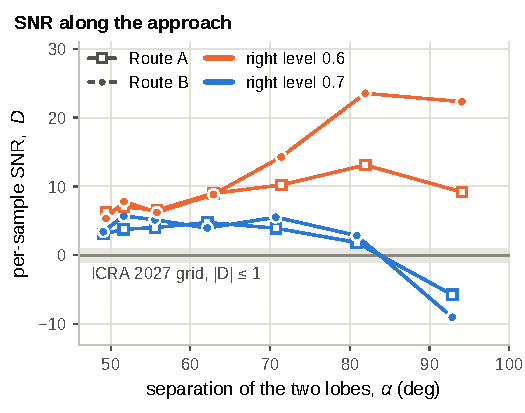
\includegraphics[width=3.5in]{fig3_snr_along_approach.pdf}
\end{minipage}\hfill
\begin{minipage}[c]{2.55in}
\caption{Per-sample SNR in blocks of seven cycles counted back from the turn, for the four runs at 0.7 that
turned right and the five runs at 0.6. A positive $D$ favours the left speaker. The grey band is the range of the
ICRA grid. Route A and Route B agree until the noise becomes small, near the turn, where Route A is held up
by what its pose model leaves unexplained.}
\label{fig:snr}
\end{minipage}
\end{figure}

Along the approach the two conditions part (Fig.~\ref{fig:snr}). At 0.6 the signal stays near 0.2 while the
noise falls, and $D$ climbs from 6 to between 9 and 23. At 0.7 $D$ stays between 3 and 6 until the lobes are
$70^\circ$ apart. Then the signal falls, passes through zero near $\alpha=84^\circ$ ($77^\circ$ to $87^\circ$ in the four runs), seven to
eleven cycles before the turn, and ends at $\dq=-0.12$ to $-0.13$: the right
lobe is now the taller one (Fig.~\ref{fig:sample}a), and $D=-5.3$ (Route A) to $-8.7$ (Route B). For a few cycles
around the crossing the input of the 0.7 runs is inside the ICRA range, on its way from one sign to the other. In A1\_11, the fifth run at 0.7, the left lobe stays taller throughout,
by 0.22 to 0.23 before the turn.

Against the ICRA grid the start values are 3.4 to 26 times larger than $D=1$ to $0.25$, and those before the
turn larger still. The ratio is large because the noise is small: the lobes differ by 13 to 19\,\%, and a lobe
height repeats from cycle to cycle within a few per cent.

\section{Why the signal drifts, and what decided the runs}

\begin{figure}[t]
\widefig{fig4_geometry.pdf}
\caption{\textbf{(a)} Logarithm of the ratio of the robot's distances to the left and right speakers, along the
approach. Every run starts 2 to 3\,\% nearer to the right speaker. \textbf{(b)} The log lobe ratio with the level
and separation terms of \eqref{eq:routeA} removed, against the log distance ratio, for three ranges of the
separation, with the fitted slopes $\gamma$. The inverse-square law would give $\gamma=2$.}
\label{fig:geometry}
\end{figure}

The lobe ratio follows the ratio of the distances to the two speakers, and steeply so
(Fig.~\ref{fig:geometry}b). The exponent $\gamma$ in \eqref{eq:routeA} is 1.6 (interval 0.2 to 3.0) at
$\alpha=50^\circ$, 3.8 (3.0 to 4.6) at $70^\circ$ and 6.5 (6.1 to 7.2) at $95^\circ$. Near the turn a change of 1\,\% in
$d_L/d_R$ changes the lobe ratio by 6.5\,\%, three times what the inverse-square law would give. There, one
centimetre of sideways displacement changes $\ln(d_L/d_R)$ by 0.022 and the lobe ratio by 14\,\%, which is the size
of the whole signal.

Every run started with the tracked robot 24 to 37\,mm nearer to the right speaker than to the left (1.21\,m against
1.24\,m). Driving straight on, such an offset grows in proportion as the distances shrink: in the three tracked runs
at 0.7 that turned right, $\ln(d_L/d_R)$ rose from 0.03 at the start to 0.06 before the turn
(Fig.~\ref{fig:geometry}a). Through $\gamma$ that raises the lobe ratio by a factor
$\exp(6.5\times0.06-1.6\times0.03)\approx1.4$, from 0.87 to about 1.2, which is what the samples show
($\bar\rho=1.15$ over the last eight cycles and 1.20 to 1.26 over the last three). At 0.6 the left lobe is taller by
19\,\% rather than 13\,\% at the start, the bump sits further to the left, and the robot drifts about 3\,cm to the left
on its way (Fig.~\ref{fig:input}b). That brings it close to equidistance, with $\ln(d_L/d_R)$ between $-0.01$ and
0.02, and the lobe ratio stays below 1. A1\_11 shows the same thing from the other side. It started 1 to 1.5\,cm further left
than the other runs and lost the right lobe in cycles 5 and 8; each time the bump followed the left lobe and the
robot turned $21^\circ$ to the left. From cycle 10 on it travelled about 2\,cm to the left of the other runs at 0.7,
within 1\,cm of equidistance from the two speakers; the left lobe stayed taller, and it turned left.

The level setting itself moves the ratio less than this geometry does. Going from 0.7 to 0.6 lowers $\ln\rho$ by
0.08 (0.06 to 0.10), about what 6\,mm of sideways displacement does near the turn. On the line equidistant from
the two speakers the model gives $\rho=0.85$ to 0.86 at 0.7 and 0.78 to 0.79 at 0.6, at both ends of the approach. Had
the robot stayed on that line, the left lobe would have remained the taller one by about 15\,\% and 21\,\%, with no
change of sign. This is an extrapolation of \eqref{eq:routeA} for the right-turning runs, and A1\_11 is the one run
that tested it. ``Equidistant'' refers to the tracked origins of the robot and the speakers, which need not be
the acoustic centres of the microphone array and the loudspeakers.

Each of the ten runs turned towards the lobe that was taller in its last three samples before the turn
(Table~\ref{tab:runs}): $\rho$ was 1.20 to 1.26 in the four that went right and 0.74 to 0.90 in the six that went
left. The ring's own randomness does not change this. Replaying each run up to its turn with 200 other seeds,
no replica turned towards the other speaker: at the cycle of the logged turn a replica had either turned the same
way or not turned yet. So the sensory
noise of Table~\ref{tab:snr} decided none of the runs. The two missing lobes of A1\_11 did change an outcome, and
they did it by moving the robot: the ring still followed the taller lobe.

\section{The noise}\label{sec:noise}

\begin{figure}[t]
\widefig{fig5_noise.pdf}
\caption{\textbf{(a)} Noise $\so$ along the approach by the two routes, in the blocks of Fig.~\ref{fig:snr}.
\textbf{(b)} Residuals of Route A in units of their robust standard deviation, with a normal curve of the same
area. \textbf{(c)} Log lobe ratio, less its running median over nine cycles, against the time of the cycle modulo
the 2-s period of a speaker's chirps, for the runs of the third sound session.}
\label{fig:noise}
\end{figure}

The noise is $\so=0.04$ to 0.05 at the start, 1.2\,m from the speakers, and falls as the robot
comes closer (Fig.~\ref{fig:noise}a). Before the turn, 0.7\,m from the speakers, Route B gives 0.011 (0.6) and 0.020
(0.7) and Route A 0.027 and 0.035.

At the start the two routes give the same noise, so it is white and the pose leaves nothing
unexplained. Before the turn Route A exceeds Route B, and the difference,
$(\sigma_A^2-\sigma_B^2)^{1/2}\approx0.025$ to 0.03, is a part of the scatter that varies slowly within a run or
differs from run to run, and that the pose model cannot place. The residuals of Route A are correspondingly
correlated from one cycle to the next (0.19 at lag one, 0.15 at lag two, within $\pm0.1$ beyond). It is the same
split as that between the white and the frozen part of the sensory stream in the paper code. At 0.025 to 0.03 it is a quarter of the signal or less.

The noise is not normal (Fig.~\ref{fig:noise}b). Of the 449 residuals of the log ratio, 15 (3.3\,\%)
lie beyond three robust standard deviations, ten on the side of a low right lobe; the excess kurtosis is 3.9. Without
those fifteen a Shapiro-Wilk test no longer rejects normality ($p=0.054$), and the standard deviation is 0.038
against 0.049 with them.

The large deviations are tied to the timing of the chirps. A speaker chirps every 2\,s and a
control cycle lasts 3.77\,s, so the listening window slides along the chirp train by 0.23\,s per cycle. In the third
sound session (A1\_08 to A1\_11) the detrended log ratio depends on the clock time modulo 2\,s
(Fig.~\ref{fig:noise}c): this phase explains 18\,\% of its variance, against 3.6\,\% expected by chance (permutation
$p=0.0002$). Ten of the twelve deviations below $-0.08$ lie at phases 0.6 to 0.9\,s, and four of the five above
$+0.08$ lie at 1.6 to 1.8\,s, one second later, which is the offset between the chirps of the two speakers. The
second session (A1\_03 to A1\_07) shows the same, more weakly (6.6\,\% against 2.8\,\%, $p=0.014$). The likely cause
is a chirp that falls at an edge of the listening window and is caught only in part; the audio that would confirm it
was not recorded.

A small part of the noise is made by the robot. The bump moves by a few
degrees from cycle to cycle, the robot turns with it, and the lobe ratio changes by 0.9\,\% per degree of that
turn. At the start this accounts for 19\,\% of the variance of the change of the log ratio from one cycle to the
next, and for 9\,\% over the whole approach.

In two of the 501 samples before the turn, both in A1\_11, the right lobe was missing: it
was below the skirt of the left lobe, that is, below 0.2. These are not part of $\so$. The cycles around them
lasted 4.0 to 5.5\,s instead of 3.8\,s, so the controller was disturbed at the time.

\section{What this means for an SNR sweep like the paper's}

The sound input sits well above the ICRA grid, and its mean depends strongly on position. To bring $D$ down to
1 with the present noise, the two lobes would have to differ by $\dq=\so/\sqrt2\approx0.03$ or less. Near the
turn that is the effect of 2 to 3\,mm of sideways displacement, so a sweep of $D$ cannot be set by the speaker
levels alone. The signal would first have to be made independent of the path: by starting on the line where the
lobes of equally driven speakers are equal, or by trimming one speaker until they are. The two levels used so
far extrapolate to equal lobes at the present start for a right level near 0.9, a rough figure from two points.
The noise can then be injected: a random factor of known spread on the amplitude of each chirp in
\code{sound\_generator\_switch.py}, or on the two lobe heights before the rescaling of \eqref{eq:h}, sets $\eta$ by
design, with the 3\,\% found here as the floor. Alternating which speaker is the louder one would separate the
effect of quality from that of side. And logging the profile $\bm{a}_n$ before rescaling, the level of each
measurement and the heading of the robot would let the next data set give the SNR directly.

\section{Checks and limits}

\begin{table}[H]
\centering\small
\caption{Checks made on the analysis.}
\label{tab:checks}
\begin{tabular}{@{}>{\raggedright\arraybackslash}p{0.49\textwidth}>{\raggedright\arraybackslash}p{0.47\textwidth}@{}}
\toprule
Check & Outcome\\
\midrule
Ring replayed from the logged inputs with seed 300 & 0 of 105\,000 spins differ; bump angles agree to $10^{-14}$ degrees\\
Clocks of the robot and of Qualisys & the robot starts to move 0.02 to 0.06\,s after the logged time\\
Robot at rest while listening & position scatter at most 0.3\,mm\\
The lobes are the speakers & lobe separation against the angle the tracked speakers subtend: $r=0.995$, lobes $3.2^\circ\pm2.2^\circ$ closer\\
Outcome read from the log against the outcome reported & 10 of 10 agree\\
Headline numbers recomputed by a separate script with another peak finder & $D_B=3.83$, 6.26, $-8.77$, 22.8 against 3.84, 6.26, $-8.69$, 23.0\\
Lobe heights from raw maxima instead of the parabola & $o_n$ changes by at most 0.002\\
Second differences instead of first, at the start & $\sigma_B=0.045$ and 0.040 against 0.048 and 0.042\\
\bottomrule
\end{tabular}
\end{table}

The checks are in Table~\ref{tab:checks}. As for the limits, the rescaling of \eqref{eq:h} removes the
absolute level, so the acoustic signal-to-noise ratio in decibels cannot be recovered from these logs; what is
measured is the SNR of the quality difference as the ring sees it, which is the quantity the paper uses. There
are five runs per level, the 0.6 runs come from one sound session and the 0.7 runs from two, and the intervals
are wide for that reason. A1\_01 has no trajectory, so Route A rests on nine runs; the tracking of A1\_10 stops
13 cycles after its turn, which affects nothing here. The model of Route A is empirical: $\alpha$ and
$\ln(d_L/d_R)$ stand in for the pose, and $\gamma$ lumps the fall of level with distance together with whatever
else changes with sideways position, such as the directivity of the speakers and of the array, and with the subtraction of the floor in \eqref{eq:h}.
Finally,
\code{ring\_circle\_target.py} in the repository is not exactly the file that ran on the robot: it names its output
differently and takes no run ID. The replay shows that its ring and the ring parameters are the same; its audio
front end cannot be checked from the logs, so the file from the robot is worth committing.

\appendix
\section{Runs and fitted parameters}

\begin{table}[H]
\centering\small
\caption{The ten runs. Turn: cycle of the turn and its side. $\rho$: lobe ratio $\qR/\qL$ over the last three
samples before the turn. Tracked: cycles before the turn with a Qualisys position. Lag: median delay between
the logged time of a cycle and the start of the robot's next move in the Qualisys record. Replicas: of 200
replays with other seeds, those that at the cycle of the turn had turned the same way, had not yet turned, or
had turned the other way.}
\label{tab:runs}
\setlength{\tabcolsep}{4.2pt}
\begin{tabular}{@{}l c c c c c c c c c c@{}}
\toprule
Run & Right & Cycles & \multicolumn{2}{c}{Turn} & $\rho$ & Tracked & Missing & Spins & Lag & Replicas: same /\\
 & level & & cycle & side & & & lobes & differing & (s) & not yet / other\\
\midrule
A1\_01 & 0.7 & 85 & 50 & R & 1.20 & 0 & 0 & 0 & n/a & 185 / 15 / 0\\
A1\_03 & 0.6 & 85 & 50 & L & 0.84 & 50 & 0 & 0 & 0.03 & 200 / 0 / 0\\
A1\_04 & 0.6 & 85 & 49 & L & 0.85 & 49 & 0 & 0 & 0.04 & 22 / 178 / 0\\
A1\_05 & 0.6 & 86 & 49 & L & 0.74 & 49 & 0 & 0 & 0.05 & 102 / 98 / 0\\
A1\_06 & 0.6 & 92 & 55 & L & 0.90 & 55 & 0 & 0 & 0.06 & 197 / 3 / 0\\
A1\_07 & 0.6 & 89 & 50 & L & 0.87 & 50 & 0 & 0 & 0.05 & 85 / 115 / 0\\
A1\_08 & 0.7 & 89 & 50 & R & 1.21 & 50 & 0 & 0 & 0.05 & 156 / 44 / 0\\
A1\_09 & 0.7 & 89 & 51 & R & 1.22 & 51 & 0 & 0 & 0.05 & 98 / 102 / 0\\
A1\_10 & 0.7 & 89 & 50 & R & 1.26 & 50 & 0 & 0 & 0.05 & 182 / 18 / 0\\
A1\_11 & 0.7 & 86 & 47 & L & 0.78 & 47 & 2 & 0 & 0.02 & 196 / 4 / 0\\
\bottomrule
\end{tabular}
\end{table}

\begin{table}[H]
\centering\small
\caption{Parameters of Route A, equation \eqref{eq:routeA}, with 95\,\% bootstrap intervals. The intercepts
$c_a$ are the log lobe ratio at equal distances and $\alpha=70^\circ$.}
\label{tab:par}
\begin{tabular}{@{}l r l@{\qquad\qquad}l r l@{}}
\toprule
Parameter & Value & Interval & Parameter & Value & Interval\\
\midrule
$c_{0.7}$ & $-$0.239 & [$-$0.257, $-$0.225] & $a_3$ & $-$0.037 & [$-$0.071, $-$0.004]\\
$c_{0.6}$ & $-$0.321 & [$-$0.346, $-$0.300] & $\gamma_0$ & 3.78 & [3.00, 4.58]\\
$a_1$ & 0.018 & [$-$0.012, 0.045] & $\gamma_1$ & 2.67 & [1.93, 3.66]\\
$a_2$ & 0.104 & [0.090, 0.129] & & & \\
\bottomrule
\end{tabular}
\end{table}

\begin{table}[H]
\centering\small
\caption{Files in \code{snr\_analysis/}. Run the two scripts from the repository root; a full run of the first
takes about four minutes.}
\label{tab:files}
\begin{tabular}{@{}>{\raggedright\arraybackslash}p{0.42\textwidth}>{\raggedright\arraybackslash}p{0.54\textwidth}@{}}
\toprule
File & Content\\
\midrule
\code{sonoro\_snr.py} & the analysis: reads \code{ringStats/} and \code{trajectories/}, writes \code{out/}\\
\code{make\_figures.py} & draws Figs~\ref{fig:input} to \ref{fig:noise} into \code{fig/}\\
\code{out/cycles.csv} & one row per control cycle: lobes, sample, geometry\\
\code{out/precommit\_samples.csv} & the samples before the turn, with fit and residual of Route A\\
\code{out/snr\_table.csv} & Table~\ref{tab:snr}, with further windows and robust variants\\
\code{out/snr\_along\_approach.csv} & the blocks of Figs~\ref{fig:snr} and \ref{fig:noise}a\\
\code{out/runs.csv}, \code{decisions.csv}, \code{seed\_replay.csv} & Table~\ref{tab:runs}\\
\code{out/route\_a\_parameters.csv} & Table~\ref{tab:par}\\
\code{out/window\_sensitivity.csv}, \code{noise\_acf.csv}, \code{noise\_phase\_locking.csv}, \code{summary.json} & checks and noise diagnostics\\
\bottomrule
\end{tabular}
\end{table}

\end{document}
